\documentclass{article}
\usepackage[utf8]{inputenc}
\usepackage[left=25mm,right=25mm,top=25mm,bottom=25mm,paper=a4paper]{geometry}
\usepackage{siunitx, amsmath,
            booktabs, tabularray,
            pdflscape, parskip, graphicx, hyperref, float}
\DeclareSIUnit\angstrom{\text{\AA}}
\UseTblrLibrary{booktabs, siunitx}

\title{Expt 2: Integral Field Spectroscopy and Galaxy Rotation Curves}
\author{Xin Cheng Liu, Student ID:22027227}
\date{}

\begin{document}
\maketitle

\section{Introduction}
\subsection{Background}
Evidence for the existence of dark matter first arose from observations and measurements of galaxy rotation curves 
of spiral galaxies in the 1970s \cite{einasto1974dynamic}\cite{ostriker1974size}\cite{roberts1973comparison}\cite{rubin1970rotation}.
The rotation curve is the rotation velocity of content around the centre of a galaxy as a function of distance from 
the centre. 

At radii close to the edge where the galaxy's luminous matter is no longer rapidly increasing, one would expect the 
rotation velocity to begin to decrease. However, in many cases, such a decrease is not observed, suggesting that 
there is additional unseen mass present. 

Measuring the velocity curve of a galaxy involves techniques using spectroscopy and the Doppler effect. The MaNGA
\cite{bundy2014overview} survey has allowed for the construction of data cubes. A two-dimensional image of a galaxy 
is obtained at each third dimensional wavelength. 

Measuring the doppler shift can be used to determine the velocity of different parts of the galaxy along
the line of sight. The most prominent emission lines in the optical spectrum of star-forming galaxies are 
is the H$\alpha$, hence, it's commonly used for making velocity measurements. However, other emission lines are
also capable of being used and the more lines that are used, the better the resulting measurement will be.


\subsection{Aims and objectives}
The aims of this project are to:
\begin{itemize}
    \item Inspect the MaNGA IFU data cube to become familiar with the data format and make some
emission line maps.
    \item Fit Gaussian models to the [NII] and H$\alpha$ emission lines in each spectrum in the data cube to
measure the redshift at that position.
    \item Convert these redshift measurements to velocity and create a velocity map.
    \item Measure the relationship between velocity and radius along the major axis of the galaxy.
    \item Make a flux map of the galaxy to determine the shape of the luminosity profile.
    \item Use the luminosity profile to estimate the expected velocity profile assuming the only mass present
comes from the stars and compare it with your measured velocity profile.
    \item Effectively communicate your approach, methods, results and their implications in the form of a
written report including data visualizations.
\end{itemize}


\section{Data description and origin}
The data used in this project is from the MaNGA survey. The data cubes contain spatially resolved spectra of
galaxies, with two spatial dimensions and one dimension for the wavelength spectrum. MaNGA (Mapping Nearby Galaxies 
at Apache Point Observatory) is an integral field spectroscopic survey of about 10,0000 nearby galaxies. Observation 
was carried out using 17 simultaneous integral field units (IFUs) and resulted in spatially resolved spectra of 
galaxies. 

A bundle of fibres is used to collect light from different regions of the galaxy, which is then brought into the
spectrograph to create a spectrum. The resulting spectra are then combined to create a data cube.

\section{Analysis and results}
\subsection{MaNGA Emission line and Flux maps}
Following the tutorial to familiarise myself with the MaNGA data cube, I plotted the wavelengths against the flux
for the central spaxel of the galaxy. The prominent emission lines are visible in Figure \ref{fig:wave}.

Following this I proceeded to create line flux maps for various emissions lines by setting bounds on the wavelength
and taking the sum of the flux within each spaxel over the specified wavelength range. The resulting maps are shown
in Figures \ref{fig:halpha} to \ref{fig:sii}.

\begin{figure}[H]
    \caption{Wave emission line map}
    \label{fig:wave}
    \centering

    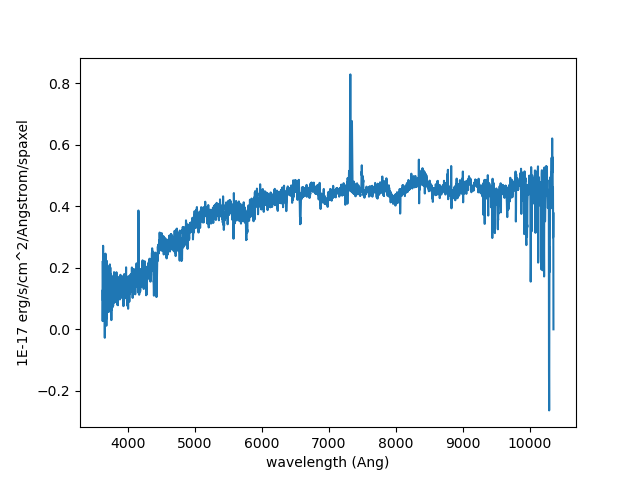
\includegraphics[width=15cm]{wave.png}
\end{figure}

\begin{figure}[H]
    \caption{H$\alpha$ flux map}
    \label{fig:halpha}
    \centering

    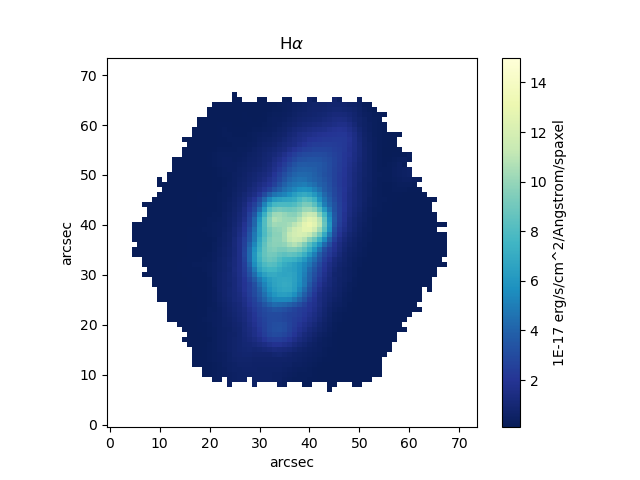
\includegraphics[width=15cm]{halpha.png}
\end{figure}

\begin{figure}[H]
    \caption{NII 1 flux map}
    \label{fig:nii1}
    \centering

    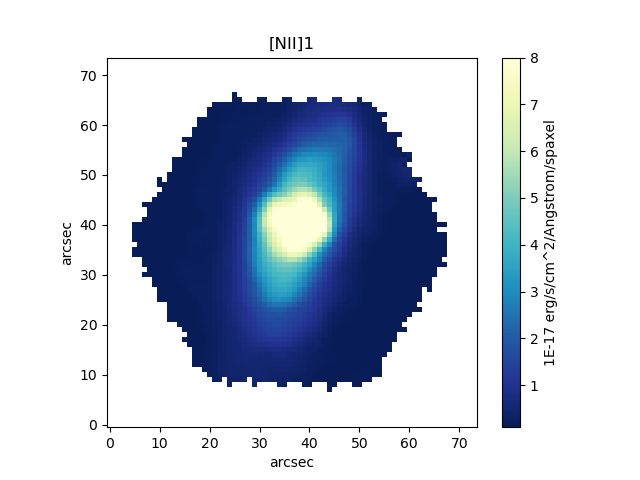
\includegraphics[width=15cm]{NII_1.png}
\end{figure}

\begin{figure}[H]
    \caption{NII 2 flux map}
    \label{fig:nii2}
    \centering

    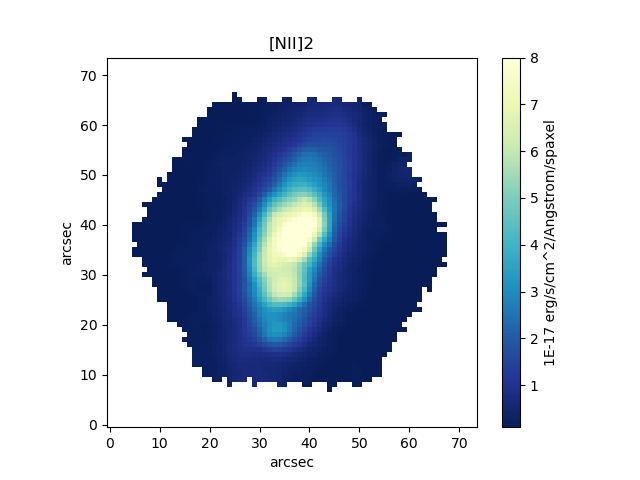
\includegraphics[width=15cm]{NII_2.png}
\end{figure}

\begin{figure}[H]
    \caption{OII flux map}
    \label{fig:oii}
    \centering

    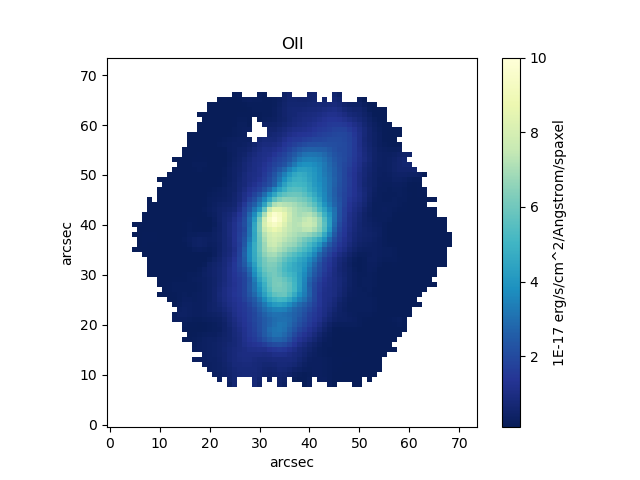
\includegraphics[width=15cm]{OII.png}
\end{figure}

\begin{figure}[H]
    \caption{OIII 1 flux map}
    \label{fig:oiii1}
    \centering

    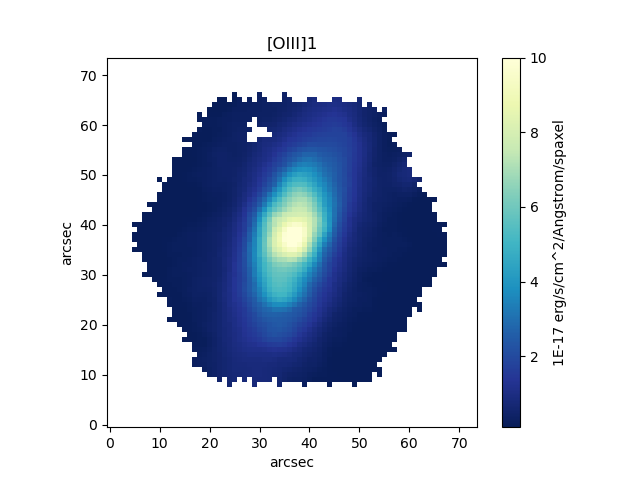
\includegraphics[width=15cm]{OIII_1.png}
\end{figure}

\begin{figure}[H]
    \caption{OIII 2 flux map}
    \label{fig:oiii2}
    \centering

    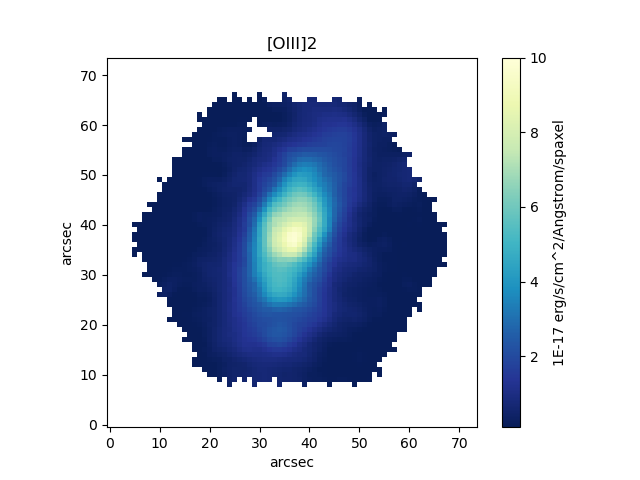
\includegraphics[width=15cm]{OIII_2.png}
\end{figure}

\begin{figure}[H]
    \caption{SII 1 flux map}
    \label{fig:sii}
    \centering

    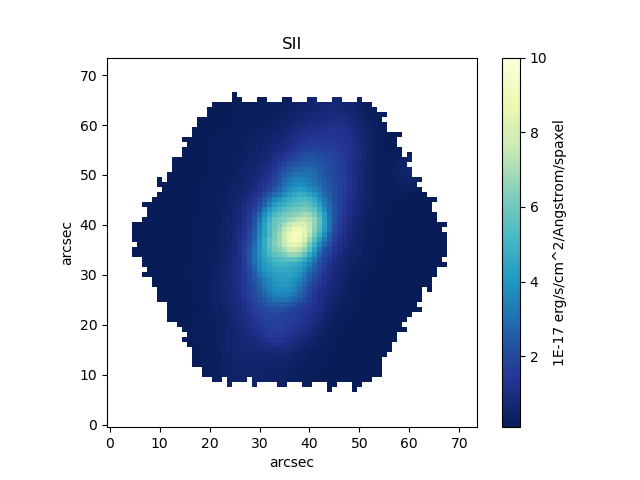
\includegraphics[width=15cm]{SII.png}
\end{figure}


\subsection{Constructing a velocity map}
To construct a velocity map, I fitted Gaussian profiles from Equation \ref{eq:gaussian fit} to the H$\alpha$ and 
[NII] emission lines. The fit is shown in Figure \ref{fig:central spaxel fit} for the central spaxel and appears to
be a good fit. This was also tested with spaxel closer towards the edge and the fit still holds up well.

\begin{equation}
    \label{eq:gaussian fit}
  \begin{split}
    \mathrm{flux}(\lambda_{\mathrm{obs}}) &= C \\[4pt]
    &\quad + A_{\mathrm{H}\alpha}
      \exp\!\left[
        -\frac{\big(\lambda_{\mathrm{obs}}
          -\lambda_{\mathrm{H}\alpha,\mathrm{rest}}(1+z)\big)^2}
        {2\sigma^2}
      \right] \\[6pt]
    &\quad + A_{[\mathrm{N\,II}]_1}
      \exp\!\left[
        -\frac{\big(\lambda_{\mathrm{obs}}
          -\lambda_{[\mathrm{N\,II}]_1,\mathrm{rest}}(1+z)\big)^2}
        {2\sigma^2}
      \right] \\[6pt]
    &\quad + A_{[\mathrm{N\,II}]_2}
      \exp\!\left[
        -\frac{\big(\lambda_{\mathrm{obs}}
          -\lambda_{[\mathrm{N\,II}]_2,\mathrm{rest}}(1+z)\big)^2}
        {2\sigma^2}
      \right]
  \end{split}
\end{equation}

\begin{figure}[H]
    \caption{Central spaxel flux-wavelength fit, }
    \label{fig:central spaxel fit}
    \centering

    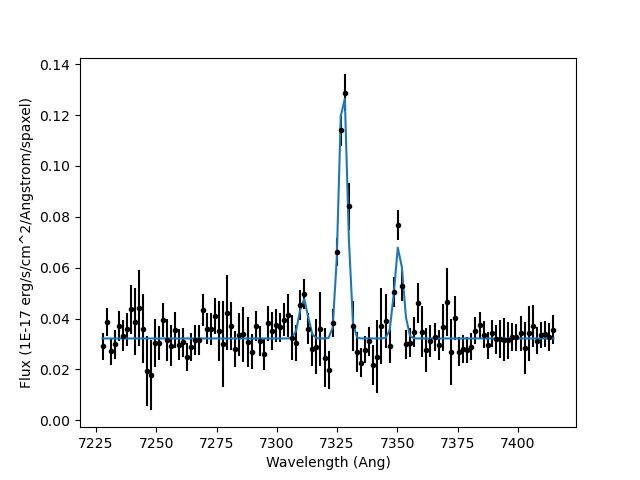
\includegraphics[width=15cm]{fluxwave.png}
\end{figure}

\begin{table}[H]
    \caption{Parameters and Errors for central spaxel flux-wavelength fit}
    \label{tab:table12}
    \centering

    \begin{tblr}{l c c c c c c}
        Parameter & C & H$\alpha$ Peak & NII 1 Peak & NII 2 Peak & Sigma & z \\
        \midrule
        Value & 0.0322 & 0.103 & 0.0157 & 0.0368 & 1.72 & 0.116 \\
        Error ($\mathbin{\substack{+\\-}}$) & 6.90e-04 & 5.92e-03 & 4.55e-03 & 4.65e-03 & 1.15e-01 & 1.74e-05 \\
        \bottomrule
    \end{tblr}
\end{table}

The errors on the flux were obtained from the data cube, taking the square root of the masked ivar data structure.
This error was used in the fitting process to weight the data points accordingly, and in turn produced suitable 
errors on the fitted parameters as well.

Once I confirmed the fit was suitable to use, I proceeded to fit the Gaussian profiles to spaxels where there was 
sufficient data. This filtering was done by using the masks provided and a signal to noise ratio cut from Equations 
\ref{eq:SN cut}. The resulting velocity map is shown in Figure \ref{fig:velocity map}.

\begin{equation}
    \label{eq:SN cut}
  \begin{aligned}
    \frac{A_{\mathrm{H}\alpha}}{\mathrm{err}\,A_{\mathrm{H}\alpha}} &> 5, \\[4pt]
    \frac{A_{[\mathrm{N\,II}]_2}}{\mathrm{err}\,A_{[\mathrm{N\,II}]_2}} &> 3, \\[4pt]
    A_{\mathrm{H}\alpha} &> 3\,\times\,\mathrm{err}\,C
  \end{aligned}
\end{equation}

\begin{figure}[H]
    \caption{velocity map}
    \label{fig:velocity map}
    \centering

    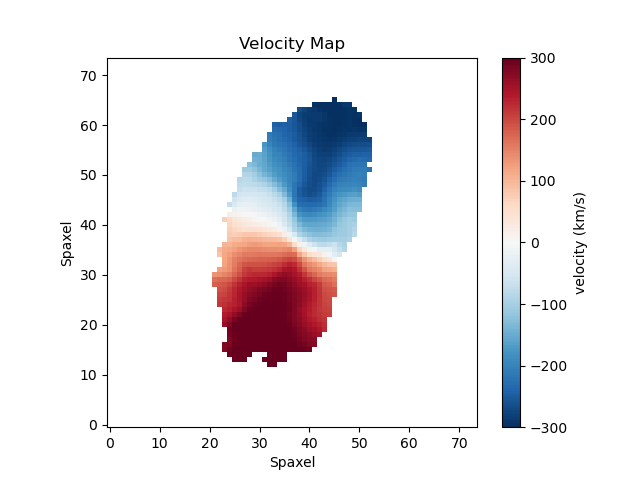
\includegraphics[width=15cm]{velocity_map.png}
\end{figure}

This velocity map partially looks as I would expect it, we can see that towards the centre of the galaxy, the 
velocity is close to zero, while towards the edge the velocity increases in magnitude but in opposite directions
on either side. This is because one side of the galaxy is moving towards us while the other side is moving away 
from us. However, I would expect the increase in velocity to begin to decrease as we approach the edge of the galaxy,
but this is not observed on the velocity map. Instead, we find the maximum velocities to be at the very edge of the
galaxy. 

In this velocity map I have used the peak lines flux to identify usable fits however, this may not be the best method
as it does not take into account the width of the lines. A better method may be to use the total flux of the lines.
I've attempted to do this by approximating a line to a isosceles triangle with a half base of $3\times\sigma$ and height 
as the peak flux in the line. Obtaining the area gives an estimation of the total flux. My conditions for usable fits 
with this method are shown in Equation \ref{eq:SN total flux}. The resulting velocity map is shown in Figure
\ref{fig:velocity map total flux}.

\begin{equation}
    \label{eq:SN total flux}
  \begin{split}
    \frac{3\times\sigma\,A_{[\mathrm{N\,II}]_2}}
         {3\times\big(\dfrac{\mathrm{err}(\sigma)}{\sigma}
          + \dfrac{\mathrm{err}A_{[\mathrm{N\,II}]_2}}{A_{[\mathrm{N\,II}]_2}}\big)}
    &> 0.05, \\[8pt]
    \frac{3\times\sigma\,A_{\mathrm{H}\alpha}}
         {3\times\big(\dfrac{\mathrm{err}(\sigma)}{\sigma}
          + \dfrac{\mathrm{err}A_{\mathrm{H}\alpha}}{A_{\mathrm{H}\alpha}}\big)}
    &> 0.10
  \end{split}
\end{equation}

\begin{figure}[H]
    \caption{Velocity map using total flux in line for S/N cut}
    \label{fig:velocity map total flux}
    \centering

    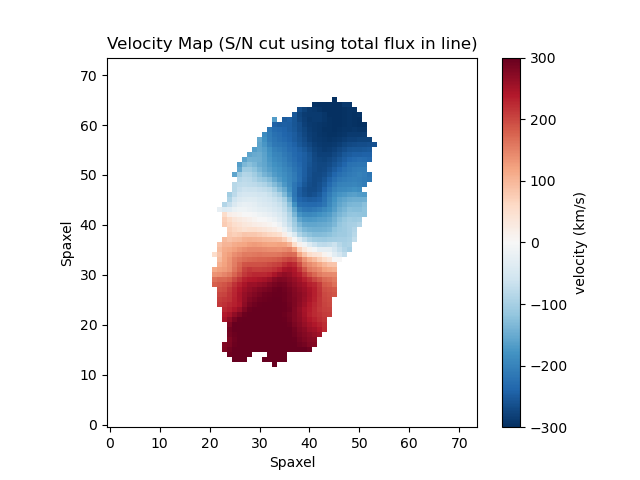
\includegraphics[width=15cm]{velocity_map_totalflux.png}
\end{figure}

\subsection{Measuring the rotation curve}
I extracted the line of sight velocity along the major axis of the galaxy and plotted it against the distance from
the central spaxel. The resulting initial rotation curve is shown in Figure \ref{fig:rotation curve}. 

I then fitted a simple model from Equation \ref{eq: rotation curve fit} to the data to obtain values for the folding 
centre position (c) , velocity centre ($0.5\times(a+d)$) and arbitrary constants in the model. The fit is shown in 
Figure \ref{fig:rotation curve fit} and appears to be a good fit.

\begin{equation}
    \label{eq: rotation curve fit}
    v_{\mathrm{los}}
    = \frac{a - d}{\,1 + \big(\tfrac{s}{c}\big)^{b}\,} + d
\end{equation}

The errors in velocity were carried over from the flux errors obtained previously during the fitting of the Gaussian
profiles. The errors of the systematic redshift was included when converting redshift to velocity (0.000019) then
multiplied by 300000 to convert to kilometers per second., during the doppler effect calculations.

\begin{equation}
  \begin{split}
    \frac{\lambda_{\mathrm{obs}} - \lambda_{r}}{\lambda_{r}}
    &= \frac{v_{\mathrm{los}}}{c}
  \end{split}
\end{equation}

After obtaining the values, I folded the rotation curve to check if the two sides of the galaxy match. The folded 
rotation curve is shown in Figure \ref{fig:rotation curve fold}. We can see that the two sides of the galaxy are 
not a perfect match but is similar enough to be considered matching.

The final step was then to correct for the inclination of the galaxy and convert the radius from spaxels to kpc.
The corrected folded rotation curve is shown in Figure \ref{fig:rotation curve fold corr}. 

\begin{figure}[H]
    \caption{rotation curve}
    \label{fig:rotation curve}
    \centering

    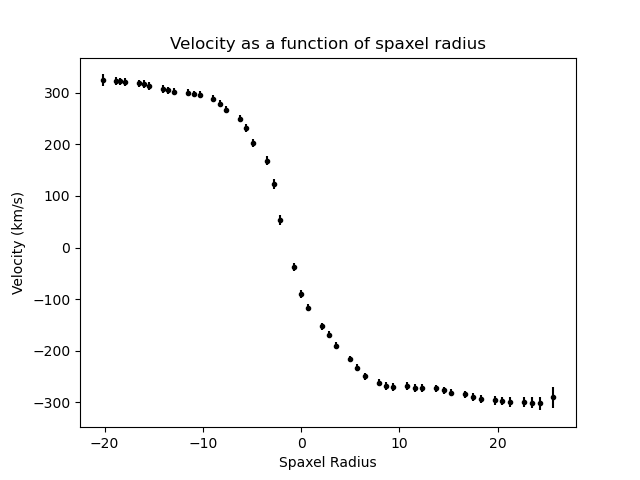
\includegraphics[width=15cm]{velocity_spaxel.png}
\end{figure}

\begin{figure}[H]
    \caption{line of sight velocity against spaxel radius fit, parameters: [a=315, b=20.3, c=52.5, d=-288]}
    \label{fig:rotation curve fit}
    \centering

    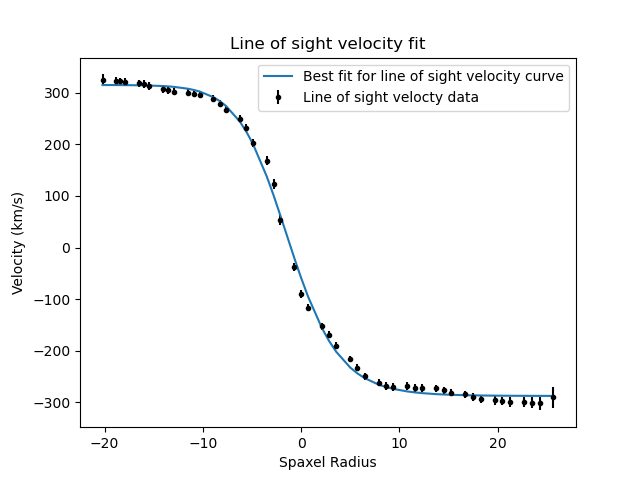
\includegraphics[width=15cm]{velocity_fit.png}
\end{figure}

\begin{figure}[H]
    \caption{rotation curve fold}
    \label{fig:rotation curve fold}
    \centering

    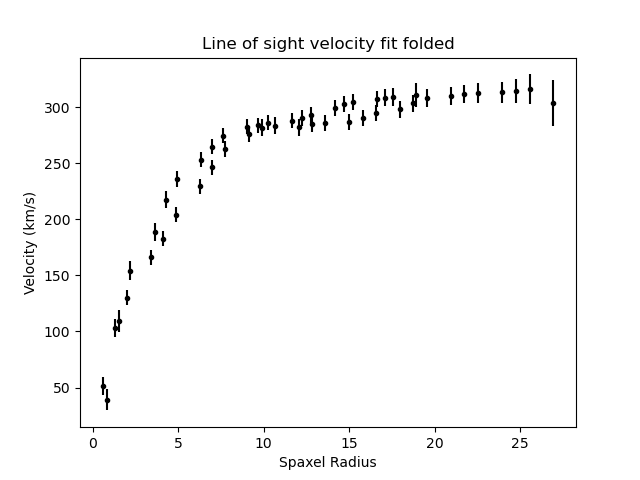
\includegraphics[width=15cm]{velocity_fold.png}
\end{figure}

\begin{figure}[H]
    \caption{rotation curve fold corrected}
    \label{fig:rotation curve fold corr}
    \centering

    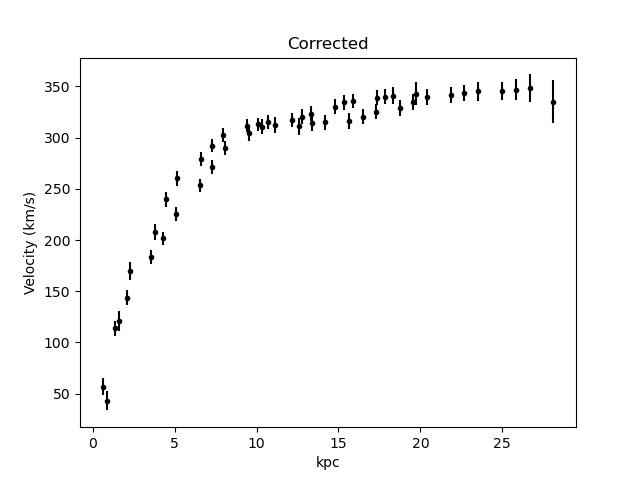
\includegraphics[width=15cm]{velocity_fold_corr.png}
\end{figure}

\subsection{Measuring flux profile and estimating rotation curve}
I first created a flux map for the wavelength range 7000 - 8000 \unit{\angstrom} by summing the flux over this range
for each spaxel. The resulting flux map is shown in Figure \ref{fig:flux map}.

Next, I measured the surface brightness along the major axis of the galaxy by summing the flux in each spaxel
along the axis. I then fitted an exponential profile to the right side of the surface brightness. The resulting 
surface brightness profile with the fit is shown in Figure \ref{fig:surface brightness}. From the fit, I obtained
parameter values for I$_0$ and R$_d$.

Using these values, I plotted the enclosed luminosity profile as a function of radius. The resulting profile is 
shown in Figure \ref{fig:encloses lum prof}.

Finally, I converted the surface brightness profile to a mass profile by assuming a mass-to-light ratio of 10,
whilst making sure all units were correct. Using this mass profile, I estimated the predicted rotation curve
using the circular velocity profile of a thin exponential disc \cite{cimatti2019introduction}. I then plotted this
with the data observed. The resulting predicted rotation curve with observed data is shown in Figure 
\ref{fig:pred rotation curve}.


\begin{figure}[H]
    \caption{Flux map for wavelengths 7000 - 8000 \unit{\angstrom}}
    \label{fig:flux map}
    \centering

    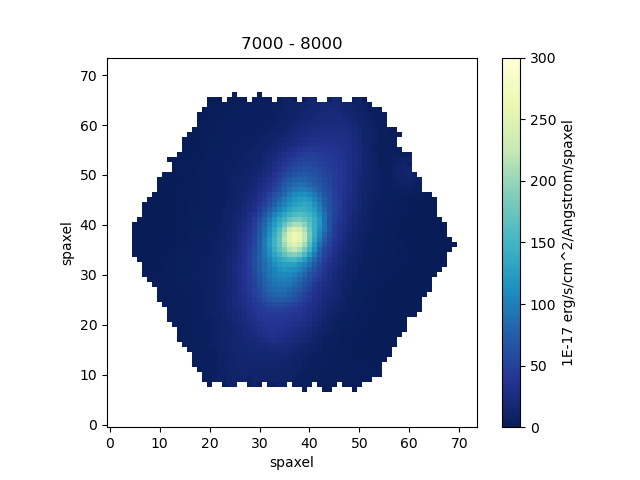
\includegraphics[width=15cm]{flux_map.png}
\end{figure}

\begin{figure}[H]
    \caption{Surface brightness along the major axis with line of best fit for right side}
    \label{fig:surface brightness}
    \centering

    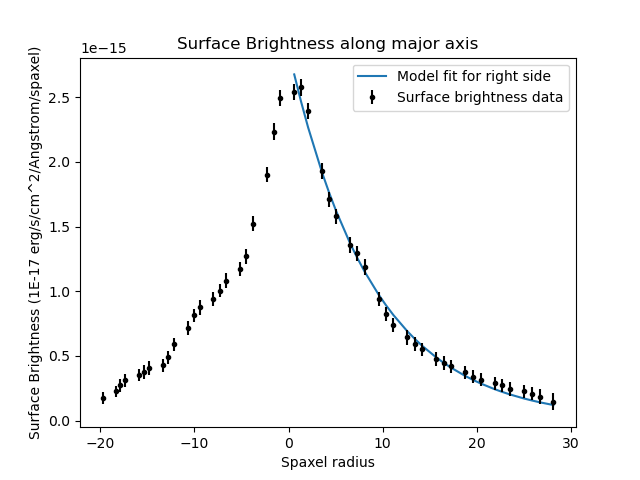
\includegraphics[width=15cm]{surface_brightness.png}
\end{figure}

\begin{figure}[H]
    \caption{Enclosed luminosity profile}
    \label{fig:encloses lum prof}
    \centering

    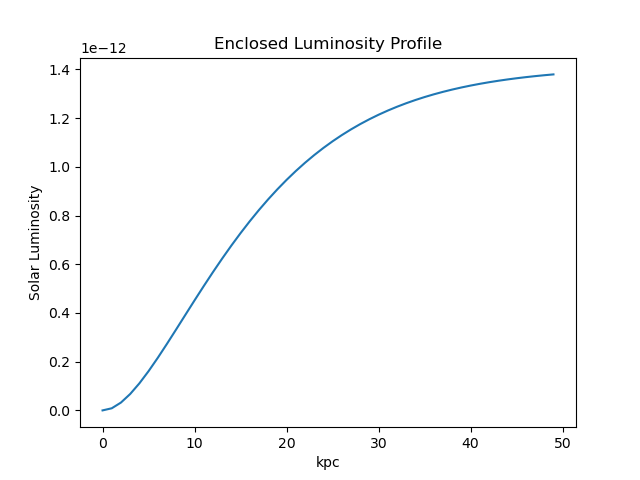
\includegraphics[width=15cm]{enclosed_lum_prof.png}
\end{figure}

\begin{figure}[H]
    \caption{Predicted rotation curve with observed data}
    \label{fig:pred rotation curve}
    \centering

    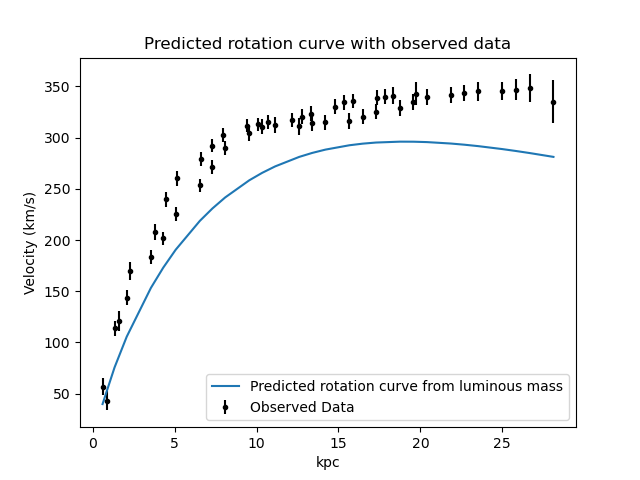
\includegraphics[width=15cm]{pred rotation curve.png}
\end{figure}

From the final predicted rotation curve with observed data, we can see that the galaxy requires dark matter. If 
our mass-to-light ratio is incorrect, the discrepancy may be explained as this ratio is our main source of
estimating the mass of the luminous components of the galaxy. An error in this ratio would lead to mistakenly
attributing the mismatch to dark matter when in fact it is due to an incorrect mass estimate.  


\section{Discussion and conclusion}
From the final predicted rotation curve with observed data, we can see that the predicted rotation curve
based on the luminous matter alone does not match the observed rotation curve. The observed rotation curve 
remains flat at large radii, while the predicted rotation curve decreases. This discrepancy suggests that there is
additional mass present in the galaxy that is not accounted for by the luminous matter alone. This additional mass
is attributed to dark matter. The presence of dark matter is necessary to explain the observed rotation curves of 
galaxies.

To improve on this analysis in the future, I would consider using more emission lines to fit the velocity
map. This would help to reduce the uncertainty in the velocity measurements and produce a more accurate velocity.
Future study could also involve analysing a larger sample of galaxies to see if the results hold across different 
types of galaxies. Additionally, I would consider using the entirety of the velocity map to construct the rotation
curve, rather than just along the major axis. This would provide a more comprehensive view of the galaxy's rotation
and help to identify any asymmetries or irregularities in the rotation curve.

\bibliographystyle{plain}
\bibliography{biblio.bib}

\end{document}
